\section{Potoki nienazwane i nazwane}
\label{sec:TQIXQ}

Współpracujące procesy i wątki mogą komunikować się ze sobą poprzez
zastosowanie mechanizmów komunikacji międzyprocesowej IPC (ang. Inter-Process
Communication). System operacyjny QNX Neutrino oferuje następujące mechanizmy
komunikacji:
\begin{myitemize}
  \item potoki (łącza) nienazwane (pipes) i nazwane (kolejki FIFO),
  \item komunikaty (message passing) i impulsy (pulses) – specyficzne dla QNX,
  \item sygnały (signals),
  \item kolejki wiadomości (message queues),
  \item pamięć współdzielona (shared memory),
  \item gniazdka (sockets).
\end{myitemize}

Niektóre z metod komunikacji są wprost implementowane w jądrze systemu
operacyjnego QNX (komunikaty i sygnały), inne stanowią zewnętrzne procesy, bądź
są częścią menadżera procesów. Projektant aplikacji może wybrać odpowiednią
metodę komunikacji, po uwzględnieniu wymagań dotyczących działania aplikacji,
takich jak:
\begin{myitemize}
  \item Czy wymagane jest stosowanie standardu POSIX?
  \item Jaka jest częstotliwość i wielkość wysyłanych wiadomości?
  \item Czy niezbędna jest komunikacja sieciowa?
  \item Czy wolno używać komunikacji blokującej?
\end{myitemize}

W tym laboratorium omówimy jeden z podstawowych rodzajów komunikacji: potoki.

\subsection{Czym jest potok?}
\label{sec:JT0OO}

Mechanizm potoków wywodzi się z~systemu UNIX i jest jedną z~najstarszych metod
komunikacji między procesami. Użytkownicy popularnych systemów operacyjnych na
ogół spotykają się z~potokami na poziomie wykonywania komend w~wierszu poleceń.
Kiedy wpisujemy sekwencję poleceń:
%%%%%%%%%%%%%%%%%%%%%%%%%%%%%%%%%%%%%%%%%%%%%%%%%%%%%%%%%%%%%%%%%%%%%%%%%%%%%
\begin{lstlisting}[style=MyBashStyle]
# cmd1 | cmd2
\end{lstlisting}
%%%%%%%%%%%%%%%%%%%%%%%%%%%%%%%%%%%%%%%%%%%%%%%%%%%%%%%%%%%%%%%%%%%%%%%%%%%%%
strumień wyjściowy procesu \texttt{cmd1} jest przekazywany na wejście procesu
\texttt{cmd2}. Przykładem użycia potoków może być wywołanie w~wierszu poleceń
następującej sekwencji:
%%%%%%%%%%%%%%%%%%%%%%%%%%%%%%%%%%%%%%%%%%%%%%%%%%%%%%%%%%%%%%%%%%%%%%%%%%%%%
\begin{lstlisting}[style=MyBashStyle]
# ls -l | wc -w
\end{lstlisting}
%%%%%%%%%%%%%%%%%%%%%%%%%%%%%%%%%%%%%%%%%%%%%%%%%%%%%%%%%%%%%%%%%%%%%%%%%%%%%

Zasada działania potoku przy ,,sprzęganiu'' komend \texttt{cmd1}
i~\texttt{cmd2}, została pokazana na rysunku \ref{fig:1CP3G}.
%%%%%%%%%%%%%%%%%%%%%%%%%%%%%%%%%%%%%%%%%%%%%%%%%%%%%%%%%%%%%%%%%%%%%%%%%%%%%
\begin{figure}[!h]
  \centering
  
\begin{tikzpicture}
    \node[draw=black]        (in1)  at (-5.50, 0.00) {KLAWIATURA};
    \node[circle,draw=black] (cmd1) at (-2.50, 0.00) {cmd1};
    \node[draw=black]        (pipe) at ( 0.00, 0.00) {POTOK};
    \node[circle,draw=black] (cmd2) at ( 2.50, 0.00) {cmd2};
    \node[draw=black]        (out2) at ( 5.50, 0.00) {MONITOR};
    \draw[->]                (in1.east)  to node[above=1ex]{stdin}  (cmd1.west);
    \draw[->]                (cmd1.east) to node[above=1ex]{stdout} (pipe.west);
    \draw[->]                (pipe.east) to node[above=1ex]{stdin}  (cmd2.west);
    \draw[->]                (cmd2.east) to node[above=1ex]{stdout} (out2.west);
  \end{tikzpicture}
  \caption{Użycie potoku do przekazywania strumieni danych}
  \label{fig:1CP3G}
\end{figure}
%%%%%%%%%%%%%%%%%%%%%%%%%%%%%%%%%%%%%%%%%%%%%%%%%%%%%%%%%%%%%%%%%%%%%%%%%%%%%
Symbole \texttt{stdin} i~\texttt{stdout} oznaczają odpowiednio wejściowy
i~wyjściowy strumień danych procesu. W~typowej sytuacji \texttt{stdin} pobiera
dane z~klawiatury a~\texttt{stdout} wyprowadza tekst na konsolę (monitor).
Użycie potoku umożliwia skierowanie strumienia \texttt{stdout} jednego procesu
do strumienia \texttt{stdin} innego procesu.

Potok jest nienazwanym plikiem, który stosuje się jako kanał komunikacyjny dla
dwóch lub więcej współpracujących procesów. Jeden z procesów pisze do potoku,
inny z niego czyta. Pojemność potoku jest ograniczona. Kiedy na przykład proces
\texttt{cmd1} pisze do potoku szybciej niż proces \texttt{cmd2} czyta, potok
może się napełnić i wtedy proces \texttt{cmd1} jest blokowany, aż do momentu,
gdy potok zostanie (przynajmniej częściowo) opróżniony przez \texttt{cmd2}.
Podobnie, gdy proces \texttt{cmd2} próbuje odebrać dane, które nie nadeszły, to
zostaje zablokowany, aż do momentu, gdy będą one dostępne.

W trakcie laboratorium poznamy niskopoziomowe funkcje dostępu do plików,
dowiemy się jaki jest wewnętrzny mechanizm przekazywania danych pomiędzy
procesami na~bazie potoków, a~także w~jaki sposób możemy zastosować potoki
do~komunikacji pomiędzy wieloma procesami.

\subsection{Niskopoziomowe funkcje dostępu do plików}
\label{sec:F6P4D}

Do obsługi potoków z~poziomu języka C można użyć niskopoziomowych funkcji
dostępu do plików. Cztery podstawowe funkcje z~tej rodziny przedstawiono
w~tabeli \ref{tab:67EKH}.
%%%%%%%%%%%%%%%%%%%%%%%%%%%%%%%%%%%%%%%%%%%%%%%%%%%%%%%%%%%%%%%%%%%%%%%%%%%%%
\begin{table}[!h]
  \centering
  \caption{Ważniejsze funkcje dostępu do plików}
  \label{tab:67EKH}
  \begin{tabular}{|l|l|}
    \hline
    \texttt{open()}   & Otwarcie lub utworzenie pliku \\ \hline
    \texttt{close()}  & Zamknięcie pliku \\ \hline
    \texttt{read()}   & Odczyt z pliku \\ \hline
    \texttt{write()}  & Zapis do pliku \\ \hline
  \end{tabular}
\end{table}
%%%%%%%%%%%%%%%%%%%%%%%%%%%%%%%%%%%%%%%%%%%%%%%%%%%%%%%%%%%%%%%%%%%%%%%%%%%%%
Typowy schemat postępowania z~plikiem sprowadza się do otwarcia pliku
(\texttt{open()}), dokonania serii odczytów/zapisów (\texttt{read()},
\texttt{write()}) a następnie zamknięcia pliku (\texttt{close()}).

Do otwarcia pliku można użyć funkcji \texttt{open()}.
%%%%%%%%%%%%%%%%%%%%%%%%%%%%%%%%%%%%%%%%%%%%%%%%%%%%%%%%%%%%%%%%%%%%%%%%%%%%%
\begin{lstlisting}[style=MyCStyle]
#include <sys/types.h>
#include <sys/stat.h>
#include <fcntl.h>

int open(const char *path, int oflags, mode_t mode);
\end{lstlisting}
%%%%%%%%%%%%%%%%%%%%%%%%%%%%%%%%%%%%%%%%%%%%%%%%%%%%%%%%%%%%%%%%%%%%%%%%%%%%%
Funkcja \texttt{open()} przyjmuje następujące argumenty:
\begin{myitemize}
  \item \texttt{path} -- ścieżka do pliku, który chcemy otworzyć,
  \item \texttt{oflags} -- flagi określające m.in. tryb dostępu do otwieranego
        pliku (tabela \ref{tab:97FHR}),
  \item \texttt{mode} -- jeśli w~argumencie \texttt{oflags} wybierzemy flagę
        \texttt{O\_CREAT}, musimy dostarczyć również zestaw parametrów
        specyfikujących prawa dostępu do nowo tworzonego pliku (tabela
        \ref{tab:VT9O5}).
\end{myitemize}
Funkcja \texttt{open()} zwraca deskryptor otwartego pliku (nieujemna liczba
całkowita) lub $-1$ w~przypadku niepowodzenia.

Flagi, których można użyć w~argumencie \texttt{oflags} przedstawiono w~tabeli
\ref{tab:97FHR}.
%%%%%%%%%%%%%%%%%%%%%%%%%%%%%%%%%%%%%%%%%%%%%%%%%%%%%%%%%%%%%%%%%%%%%%%%%%%%%
\begin{table}[!h]
  \centering
  \caption{Wybrane flagi, które można przekazać przez argument \texttt{oflags}}
  \label{tab:97FHR}
  \begin{tabular}{|l|l|}
    \hline
    \textbf{Flaga}      & \textbf{Opis} \\ \hline
    \texttt{O\_RDONLY}  & otwarcie tylko do odczytu \\ \hline
    \texttt{O\_RDWR}    & otwarcie dla odczytu i~zapisu \\ \hline
    \texttt{O\_WRONLY}  & otwarcie tylko do zapisu \\ \hline
    \texttt{O\_CREAT}   & utworzenie pliku, gdy nie istnieje \\ \hline
    \texttt{O\_APPEND}  & dopisywanie na końcu istniejącego pliku \\ \hline
    \texttt{O\_NONBLOC} & zapis i odczyt będą działać nieblokująco \\ \hline
  \end{tabular}
\end{table}
%%%%%%%%%%%%%%%%%%%%%%%%%%%%%%%%%%%%%%%%%%%%%%%%%%%%%%%%%%%%%%%%%%%%%%%%%%%%%

Flagi, których można użyć w~argumencie \texttt{mode} przedstawiono w~tabeli
\ref{tab:VT9O5}.
%%%%%%%%%%%%%%%%%%%%%%%%%%%%%%%%%%%%%%%%%%%%%%%%%%%%%%%%%%%%%%%%%%%%%%%%%%%%%
\begin{table}[!h]
  \centering
  \caption{Wybrane flagi, które można przekazać przez argument \texttt{mode}.
           Umożliwiają one zdefiniowanie praw dostępu do nowo tworzonego pliku
           (\texttt{O\_CREAT}) odpowiednio dla właściciela pliku, członków
           wyróżnionej grupy oraz pozostałych użytkowników}
  \label{tab:VT9O5}
  \begin{tabular}{|l|l|l|l|}
    \hline
    \textbf{User}     & \textbf{Group}    & \textbf{Others}   & \textbf{Permission} \\ \hline
    \texttt{S\_IRUSR} & \texttt{S\_IRGRP} & \texttt{S\_IROTH} & \texttt{r}          \\ \hline
    \texttt{S\_IWUSR} & \texttt{S\_IWGRP} & \texttt{S\_IWOTH} & \texttt{w}          \\ \hline
    \texttt{S\_IXUSR} & \texttt{S\_IXGRP} & \texttt{S\_IXOTH} & \texttt{x}          \\ \hline
    \texttt{S\_IRWXU} & \texttt{S\_IRWXG} & \texttt{S\_IRWXO} & \texttt{rwx}        \\ \hline
  \end{tabular}
\end{table}
%%%%%%%%%%%%%%%%%%%%%%%%%%%%%%%%%%%%%%%%%%%%%%%%%%%%%%%%%%%%%%%%%%%%%%%%%%%%%

Aby zamknąć plik, używamy funkcji \texttt{close()}:
%%%%%%%%%%%%%%%%%%%%%%%%%%%%%%%%%%%%%%%%%%%%%%%%%%%%%%%%%%%%%%%%%%%%%%%%%%%%%k
\begin{lstlisting}[style=MyCStyle]
#include <unistd.h>

int close(int filedes);
\end{lstlisting}
%%%%%%%%%%%%%%%%%%%%%%%%%%%%%%%%%%%%%%%%%%%%%%%%%%%%%%%%%%%%%%%%%%%%%%%%%%%%%
Funkcja \texttt{close()} przyjmuje jeden argument:
\begin{myitemize}
  \item \texttt{filedes} -- deskryptor pliku do zamknięcia, ten sam, który był
        zwrócony przez funkcję \texttt{open()}.
\end{myitemize}

Odczyt danych z~pliku realizujemy przez wywołanie funkcji \texttt{read()}
%%%%%%%%%%%%%%%%%%%%%%%%%%%%%%%%%%%%%%%%%%%%%%%%%%%%%%%%%%%%%%%%%%%%%%%%%%%%%k
\begin{lstlisting}[style=MyCStyle]
#include <unistd.h>

ssize_t read(int filedes, void *buf, size_t nbyte);
\end{lstlisting}
%%%%%%%%%%%%%%%%%%%%%%%%%%%%%%%%%%%%%%%%%%%%%%%%%%%%%%%%%%%%%%%%%%%%%%%%%%%%%
Argumenty przyjmowane przez funkcję \texttt{read()} to:
\begin{myitemize}
  \item \texttt{filedes} -- deskryptor otwartego pliku, z~którego chcemy czytać,
  \item \texttt{buf} -- wskaźnik do bufora, do którego funkcja ma zapisać przeczytane dane,
  \item \texttt{nbyte} -- liczba bajtów, którą chcemy przeczytać.
\end{myitemize}
Funkcja \texttt{read()} odczytuje \texttt{nbyte} bajtów z~pliku określonego
przez deskryptor \texttt{filedes} i~umieszcza dane w~buforze wskazywanym przez
\texttt{buf}. Gdy wywołanie funkcji się powiedzie, funkcja zwraca liczbę
przeczytanych bajtów umieszczonych w~buforze. W~przypadku błędu, funkcja zwraca
$-1$. Liczba bajtów zwracana przez funkcję może być mniejsza od \texttt{nbyte}
w~następujących przypadkach
\begin{myitemize}
  \item liczba bajtów w~pliku jest mniejsza niż \texttt{nbyte},
  \item działanie funkcji \texttt{read()} zostało przerwane przez sygnał,
  \item plik jest potokiem i~posiada w~danym momencie mniej bajtów danych niż
        \texttt{nbyte}.
\end{myitemize}

Zapis danych do pliku realizujemy poprzez wywołanie funkcji \texttt{write()}
%%%%%%%%%%%%%%%%%%%%%%%%%%%%%%%%%%%%%%%%%%%%%%%%%%%%%%%%%%%%%%%%%%%%%%%%%%%%%k
\begin{lstlisting}[style=MyCStyle]
#include <unistd.h>

ssize_t read(int filedes, const void *buf, size_t nbyte);
\end{lstlisting}
%%%%%%%%%%%%%%%%%%%%%%%%%%%%%%%%%%%%%%%%%%%%%%%%%%%%%%%%%%%%%%%%%%%%%%%%%%%%%
Argumenty przyjmowane przez funkcję \texttt{write()} to:
\begin{myitemize}
  \item \texttt{filedes} -- deskryptor otwartego pliku, do~którego chcemy pisać,
  \item \texttt{buf} -- wskaźnik do bufora w~pamięci, z którego funkcja czerpie
        dane przeznaczone do zapisu,
  \item \texttt{nbyte} -- liczba bajtów, którą chcemy zapisać.
\end{myitemize}
Funkcja \texttt{write()} zapisuje \texttt{nbyte} bajtów do pliku określonego
przez deskryptor \texttt{filedes} z~bufora wskazywanego przez \texttt{buf}.
Jeśli flaga \texttt{O\_APPEND} była ustawiona podczas otwierania pliku, to dane
są dopisywane na końcu istniejącego pliku. W przeciwnym przypadku zapis do
pliku następuje od miejsca wskazanego przez bieżącą pozycję pliku. Po dokonaniu
zapisu, wskaźnik bieżącej pozycji jest przesuwany o~liczbę zapisanych bajtów.
Liczba zapisanych bajtów może być mniejsza niż \texttt{nbyte} gdy:
\begin{myitemize}
  \item brakuje miejsca na nośniku,
  \item działanie funkcji \texttt{write()} zostało przerwane przez sygnał.
\end{myitemize}


%%%%%%%%%%%%%%%%%%%%%%%%%%%%%%%%%%%%%%%%%%%%%%%%%%%%%%%%%%%%%%%%%%%%%%%%%%%%%k
\begin{example}{[Utworzenie nowego pliku i~pisanie do pliku]}
  Uruchomić program, który tworzy nowy plik i~zapisuje do niego dane. Jako
  argument wywołania podać nazwę pliku.
  \lstinputlisting[style=MyCStyle,label=src:FXPNJ]{src/lab7/write1.c}
\end{example}
%%%%%%%%%%%%%%%%%%%%%%%%%%%%%%%%%%%%%%%%%%%%%%%%%%%%%%%%%%%%%%%%%%%%%%%%%%%%%k

%%%%%%%%%%%%%%%%%%%%%%%%%%%%%%%%%%%%%%%%%%%%%%%%%%%%%%%%%%%%%%%%%%%%%%%%%%%%%k
\begin{example}{[Kopiowanie plików]}
  Uruchomić program. Jako argumenty wywołania podać nazwę pliku do skopiowania,
  nazwę pliku docelowego i~liczbę bajtów do skopiowania.
  \lstinputlisting[style=MyCStyle,label=src:DNAMC]{src/lab7/copy1.c}
\end{example}
%%%%%%%%%%%%%%%%%%%%%%%%%%%%%%%%%%%%%%%%%%%%%%%%%%%%%%%%%%%%%%%%%%%%%%%%%%%%%k

\subsection{Potoki nienazwane}
\label{sec:NAMCF}

Komunikacja za pomocą potoków nienazwanych ma zastosowanie do procesów
pozostających w~relacji pokrewieństwa (np. proces potomny i~macierzysty). Przy
tworzeniu potoku nienazwanego tworzone są deskryptory plików reprezentujących
potok, które są dziedziczone przez procesy potomne. Komunikacja jest
jednokierunkowa. Deskryptor, który jest nieużywany przez dany proces, powinien
być w~przez ten proces zamknięty.

Utworzenie potoku wymaga wywołania funkcji \texttt{pipe()}:
%%%%%%%%%%%%%%%%%%%%%%%%%%%%%%%%%%%%%%%%%%%%%%%%%%%%%%%%%%%%%%%%%%%%%%%%%%%%%k
\begin{lstlisting}[style=MyCStyle]
#include <unistd.h>
int pipe(int filedes[2]);
\end{lstlisting}
%%%%%%%%%%%%%%%%%%%%%%%%%%%%%%%%%%%%%%%%%%%%%%%%%%%%%%%%%%%%%%%%%%%%%%%%%%%%%k
Funkcja \texttt{pipe} przyjmuje jeden argument
\begin{myitemize}
  \item \texttt{filedes} -- tablica przechowująca deskryptory plików do odczytu
        i~zapisu (końcówki potoku).
\end{myitemize}
Funkcja zwraca zero, gdy operacja się powiedzie, bądź $-1$ w~przeciwnym
przypadku. Element \texttt{filedes[0]} jest deskryptorem ,,pliku'' do odczytu
z~potoku, element \texttt{filedes[1]} jest deskryptorem ,,pliku'' do zapisu.
Operacje odczytu i~zapisu można przeprowadzić przy użyciu opisanych wcześniej
funkcji \texttt{read()} i \texttt{write()}. Zasadę działania potoku
nienazwanego przedstawiono na rysunku \ref{fig:OF6P4}.
%%%%%%%%%%%%%%%%%%%%%%%%%%%%%%%%%%%%%%%%%%%%%%%%%%%%%%%%%%%%%%%%%%%%%%%%%%%%%
\begin{figure}[!h]
  \centering
  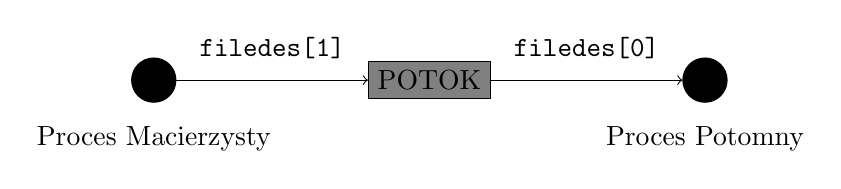
\begin{tikzpicture}
    \node[circle,draw=black,fill=black] (proc1)   at (-3.50, 0.00) {o};
    \node[draw=black,fill=gray]         (pipe)    at ( 0.00, 0.00) {POTOK};
    \node[circle,draw=black,fill=black] (proc2)   at ( 3.50, 0.00) {o};
    \node[]                             (proc1t)  at (-3.50,-0.75)  {Proces Macierzysty};
    \node[]                             (proc2t)  at ( 3.50,-0.75)  {Proces Potomny};
    \draw[->]                (proc1.east) to node[above=1ex]{\texttt{filedes[1]}} (pipe.west);
    \draw[->]                (pipe.east) to node[above=1ex]{\texttt{filedes[0]}}  (proc2.west);
  \end{tikzpicture}
  \caption{Użycie potoku do przekazywania strumieni danych}
  \label{fig:OF6P4}
\end{figure}
%%%%%%%%%%%%%%%%%%%%%%%%%%%%%%%%%%%%%%%%%%%%%%%%%%%%%%%%%%%%%%%%%%%%%%%%%%%%%

System QNX zarządza potokami poprzez menadżera potoków. Menadżer potoków
przydziela ograniczoną pamięć dla łącza danych. Bufor ten domyślnie ma rozmiar
5120 bajtów. Funkcją umożliwiającą pobranie informacji o~zmiennych
konfiguracyjnych dotyczących plików (w~tym potoków) jest \texttt{fpathconf(int
filedes, int name)}, gdzie \texttt{filedes} jest deskryptorem pliku, a
\texttt{name} jest kodem numerycznym stanowiącym nazwę odpytywanej zmiennej. W
naszym przypadku \texttt{name = \_PC\_PIPE\_BUF}.

%%%%%%%%%%%%%%%%%%%%%%%%%%%%%%%%%%%%%%%%%%%%%%%%%%%%%%%%%%%%%%%%%%%%%%%%%%%%%
\begin{example}{[Potoki nienazwane w~obrębie jednego procesu]}
  Uruchomić program. Przetestować rozmiar bufora \texttt{BUFSIZE} równy $8$.
  Zwrócić uwagę na fakt, że komunikaty czytane są w~kolejności, w~jakiej
  zostały zapisane (na bazie FIFO).
  \lstinputlisting[style=MyCStyle,label=src:QJT0O]{src/lab7/pipe1.c}
\end{example}
%%%%%%%%%%%%%%%%%%%%%%%%%%%%%%%%%%%%%%%%%%%%%%%%%%%%%%%%%%%%%%%%%%%%%%%%%%%%%

%%%%%%%%%%%%%%%%%%%%%%%%%%%%%%%%%%%%%%%%%%%%%%%%%%%%%%%%%%%%%%%%%%%%%%%%%%%%%
\begin{example}{[Potoki nienazwane w~obrębie procesu macierzystego i~potomnego (fork)]}
  Uruchomić program, w~którym proces macierzysty pisze do potoku, natomiast
  proces potomny odczytuje dane z~potoku.
  \lstinputlisting[style=MyCStyle,label=src:4TQIX]{src/lab7/pipe2.c}
\end{example}
%%%%%%%%%%%%%%%%%%%%%%%%%%%%%%%%%%%%%%%%%%%%%%%%%%%%%%%%%%%%%%%%%%%%%%%%%%%%%

Proces potomny może wywołać funkcję z~rodziny \texttt{exec()}, która zastępuje
bieżący proces innym procesem. Możliwa jest wtedy komunikacja pomiędzy procesem
macierzystym, a nowo wywołanym procesem. Jednak wywołany proces nie dziedziczy
od macierzystego deskryptorów plików, zatem musimy mu je przekazać jako
parametry wywołania procesu. Sytuację tę ilustruje przykład \ref{ex:MLOE9}.
%%%%%%%%%%%%%%%%%%%%%%%%%%%%%%%%%%%%%%%%%%%%%%%%%%%%%%%%%%%%%%%%%%%%%%%%%%%%%
\begin{example}{[Potoki nienazwane i~funkcja \texttt{exec()}]}
  \label{ex:MLOE9}
  Skompilować i~uruchomić program \textbf{konsument.c} i~\textbf{producent.c}.
  \lstinputlisting[style=MyCStyle,label=src:EZI8J]{src/lab7/konsument.c}
  \lstinputlisting[style=MyCStyle,label=src:LNIZJ]{src/lab7/producent.c}
\end{example}
%%%%%%%%%%%%%%%%%%%%%%%%%%%%%%%%%%%%%%%%%%%%%%%%%%%%%%%%%%%%%%%%%%%%%%%%%%%%%

Do tej pory mieliśmy do czynienia z~sytuacją, gdy komunikujące się procesy
wymieniały informacje bez udziału standardowych strumieni. Często wygodnie jest
połączyć deskryptory plików, uzyskane z~funkcji \texttt{pipe()} ze standardowym
wejściem $0$ oraz standardowym wyjściem $1$. Aby to zrobić, potrzebujemy dwóch
spokrewnionych ze~sobą funkcji, które umożliwiają duplikowanie deskryptorów
plików:
%%%%%%%%%%%%%%%%%%%%%%%%%%%%%%%%%%%%%%%%%%%%%%%%%%%%%%%%%%%%%%%%%%%%%%%%%%%%%
\begin{lstlisting}[style=MyCStyle]
#include <unistd.h>
int dup( int filedes );
int dup2( int filedes, int filedes 2);
\end{lstlisting}
%%%%%%%%%%%%%%%%%%%%%%%%%%%%%%%%%%%%%%%%%%%%%%%%%%%%%%%%%%%%%%%%%%%%%%%%%%%%%
gdzie
\begin{myitemize}
  \item \texttt{filedes} -- deskryptor pliku, który chcemy zduplikować,
  \item \texttt{filedes2} -- nowy deskryptor pliku, który chcemy przypisać do \texttt{filedes}.
\end{myitemize}

Nowy deskryptor wskazuje na obiekt \texttt{filedes}, przekazany jako argument
wywołania funkcji. W~szczególności ma te same atrybuty i~tryby dostępu, jak
również wskazuje na tę samą pozycję w~pliku. Funkcja \texttt{dup()}
automatycznie generuje wartość nowego deskryptora pliku (duplikatu). Funkcja
\texttt{dup2()} pozostawia to zadanie programiście, tj. programista dostarcza
nowy deskryptor jako \texttt{filedes2}. Gdy deskryptor \texttt{filedes2} jest
już otwarty, wskazywany przez niego plik zostanie najpierw zamknięty.

W dalszych przykładach skojarzymy końce potoku nienazwanego ze strumieniami
\texttt{stdin} i~\texttt{stdout}. Zabieg taki umożliwia realizację z~poziomu
języka C wywołania sekwencji procesów w~postaci
\begin{lstlisting}[style=MyBashStyle]
# program1 | program2
\end{lstlisting}

%%%%%%%%%%%%%%%%%%%%%%%%%%%%%%%%%%%%%%%%%%%%%%%%%%%%%%%%%%%%%%%%%%%%%%%%%%%%%
\begin{example}{[Potoki nienazwane i~przekierowania strumieni]}
  Skompilować, uruchomić i~przeanalizować program. Porównać wynik programu
  z~wywołaniem: \texttt{ls -l | wc -w}
  \lstinputlisting[style=MyCStyle,label=src:7FHR6]{src/lab7/redirect1.c}
\end{example}
%%%%%%%%%%%%%%%%%%%%%%%%%%%%%%%%%%%%%%%%%%%%%%%%%%%%%%%%%%%%%%%%%%%%%%%%%%%%%

Mechanizm potoków nienazwanych jest dość skomplikowany. Programista musi dbać
o~tworzenie potoków (\texttt{pipe()}), zarządzanie procesami (\texttt{fork()},
\texttt{exec()}), czy przekierowanie strumieni standardowych (\texttt{dup2()}).
Istnieją funkcje, które ułatwiają ten proces. Należą do nich \texttt{popen()}
i~\texttt{pclose()}.
%%%%%%%%%%%%%%%%%%%%%%%%%%%%%%%%%%%%%%%%%%%%%%%%%%%%%%%%%%%%%%%%%%%%%%%%%%%%%
\begin{lstlisting}[style=MyCStyle]
FILE* popen( const char *command, const char *mode );
\end{lstlisting}
%%%%%%%%%%%%%%%%%%%%%%%%%%%%%%%%%%%%%%%%%%%%%%%%%%%%%%%%%%%%%%%%%%%%%%%%%%%%%
gdzie
\begin{myitemize}
  \item \texttt{command} -- komenda, którą chcemy uruchomić jako proces potomny,
  \item \texttt{mode} -- tryb otwierania potoku (\texttt{\char`\"r\char`\"}, bądź \texttt{\char`\"w\char`\"}).
\end{myitemize}
Funkcja \texttt{popen()} uruchamia proces wskazany przez \texttt{command}
i~tworzy potok między procesem wywołującym a~procesem \texttt{command}.
W~zależności od ustawionego trybu, zwracany wskaźnik na strukturę \texttt{FILE}
może być użyty do odczytu bądź zapisu. W~przypadku błędu, funkcja zwraca
\texttt{NULL}.

Aby zamknąć potok stowarzyszony ze strumieniem \texttt{stream} używamy funkcji
\texttt{pclose()}:
%%%%%%%%%%%%%%%%%%%%%%%%%%%%%%%%%%%%%%%%%%%%%%%%%%%%%%%%%%%%%%%%%%%%%%%%%%%%%
\begin{lstlisting}[style=MyCStyle]
FILE* pclose( FILE* stream );
\end{lstlisting}
%%%%%%%%%%%%%%%%%%%%%%%%%%%%%%%%%%%%%%%%%%%%%%%%%%%%%%%%%%%%%%%%%%%%%%%%%%%%%
gdzie
\begin{myitemize}
  \item \texttt{stream} -- wskaźnik na strumień otwarty wcześniej funkcją \texttt{popen()}.
\end{myitemize}
Funkcja \texttt{pclose()} zamyka potok i~jednocześnie czeka na zakończenie
podprocesów utworzonych przez \texttt{popen()}. Funkcja zwraca status
zakończenie, bądź $-1$, w przypadku błędu.

\begin{example}{[Przykład pisania do potoku nienazwanego \texttt{popen()}, \texttt{pclose()}]}
  Skompilować, uruchomić program.
  \lstinputlisting[style=MyCStyle,label=src:7EKH1]{src/lab7/popen1.c}
\end{example}

\subsection{Potoki nazwane}
\label{sec:XPNJV}

Potoki nazwane, określane również mianem plików FIFO, pozwalają na uniknięcie
ograniczeń, którymi obarczone są potoki nienazwane. Pliki FIFO istnieją
w~przestrzeni nazw plików i~mają atrybuty, prawa dostępu, właścicieli, takie,
jak zwykłe pliki. Do obsługi potoków nazwanych używa się głównie funkcji
plikowych, jedyna różnica, to inicjalizacja potoku:
%%%%%%%%%%%%%%%%%%%%%%%%%%%%%%%%%%%%%%%%%%%%%%%%%%%%%%%%%%%%%%%%%%%%%%%%%%%%%
\begin{lstlisting}[style=MyCStyle]
#include <sys/types.h>
#include <sys/stat.h>

int mkfifo( const char* path, mode_t mode );
\end{lstlisting}
%%%%%%%%%%%%%%%%%%%%%%%%%%%%%%%%%%%%%%%%%%%%%%%%%%%%%%%%%%%%%%%%%%%%%%%%%%%%%
Funkcja \texttt{mkfifo()} przyjmuje następujące argumenty
\begin{myitemize}
  \item \texttt{path} -- nazwa pliku FIFO,
  \item \texttt{mode} -- prawa dostępu do pliku.
\end{myitemize}
Funkcja \texttt{mkfifo()} tworzy nowy plik specjalny FIFO o~nazwie podanej
przez parametr \texttt{path}. Plik FIFO będzie miał uprawnienia określone przez
argument \texttt{mode}. Funkcja zwraca $0$ w~przypadku powodzenia i~$-1$
w~przypadku błędu.

Otwieranie (\texttt{open()}) pliku FIFO do zapisu blokuje proces bieżący do
czasu, gdy inny proces nie otworzy tego pliku do odczytu. Podobna sytuacja ma
miejsce, gdy proces otwiera plik do odczytu -- jest on blokowany dotąd, aż inny
proces otworzy plik do zapisu. Możliwe jest także nieblokujące wywołanie
funkcji \texttt{open()} dla pliku FIFO (należy użyć flagi \texttt{O\_NONBLOCK}).

\begin{example}{[Tworzenie i~używanie plików FIFO z~wiersza poleceń]}
\begin{lstlisting}[style=MyBashStyle]
# mkfifo /tmp/fifo
# ls -l /tmp/fifo
prw-rw-r--  1 root root 0 Sep 12 12:24 fifo
\end{lstlisting}
Litera \textbf{p} w~atrybutach (\texttt{prw-rw-r}) oznacza, że jest to potok
nazwany (named pipe). Plik FIFO moze być odczytywany i~zapisywany za~pomocą
standardowych poleceń.
\end{example}

\begin{example}{[Zapis/odczyt pliku FIFO z~wiersza poleceń]}
Używając dwu konsoli wpisać następujące polecenia:

Konsola 1:
\begin{lstlisting}[style=MyBashStyle]
# cat < /tmp/fifo
\end{lstlisting}

Konsola 2:
\begin{lstlisting}[style=MyBashStyle]
# cat > /tmp/fifo
\end{lstlisting}

Wpisać w~konsoli 2 kilka linii tekstu i zakończyć pisanie (Ctl+D). Przełączyć
się na konsolę 1 i obejrzeć rezultat. Zakończyć polecenie na konsoli 1 (Ctl+C).
Usunąć plik FIFO jak zwykły plik.
\end{example}

Pliki FIFO można oczywiście obsługiwać z~poziomu języka C. Poniższy przykład
ilustruje sposób tworzenia, otwierania i~zamykania pliku FIFO.
%%%%%%%%%%%%%%%%%%%%%%%%%%%%%%%%%%%%%%%%%%%%%%%%%%%%%%%%%%%%%%%%%%%%%%%%%%%%%
\begin{example}{[Tworzenie i~używanie potoków nazwanych w~C]}
  Uruchomić program z~argumentami wywołania \texttt{O\_RDONLY} lub
  \texttt{O\_WRONLY}. Zaobserwować zachowanie się procesu. Sprawdzić obecność
  pliku FIFO w~systemie plików po wywołaniu programu. Uruchomić program w~dwóch
  konsolach, w pierwszej z~flagą \texttt{O\_RDONLY}, w~drugiej z~flagą
  \texttt{O\_WRONLY}. Sprawdzić co się stanie, gdy do flag dodamy opcję
  \texttt{O\_NONBLOCK}.
  \lstinputlisting[style=MyCStyle,label=src:5A3PM]{src/lab7/fifo1.c}
\end{example}
%%%%%%%%%%%%%%%%%%%%%%%%%%%%%%%%%%%%%%%%%%%%%%%%%%%%%%%%%%%%%%%%%%%%%%%%%%%%%

Następny przykład jest ilustracją zastosowania potoków nazwanych do
implementacji bardzo prostego jednokierunkowgo komunikatora. W~przykładzie mamy
proces-serwer, który odbiera komunikaty od klienta i wyprowadza je na
standardowe wyjście. Programy tworzą szkielet prostego systemu buforowania.
%%%%%%%%%%%%%%%%%%%%%%%%%%%%%%%%%%%%%%%%%%%%%%%%%%%%%%%%%%%%%%%%%%%%%%%%%%%%%
\begin{example}{[Prosty system buforowania na~bazie potoków nazwanych]}
  Skompilować, uruchomić i~przeanalizować działanie klienta i serwera.
  \lstinputlisting[style=MyCStyle,label=src:CP3GC]{src/lab7/client1.c}
  \lstinputlisting[style=MyCStyle,label=src:5RXYW]{src/lab7/server1.c}
\end{example}
%%%%%%%%%%%%%%%%%%%%%%%%%%%%%%%%%%%%%%%%%%%%%%%%%%%%%%%%%%%%%%%%%%%%%%%%%%%%%

\subsection{Ćwiczenia}
\label{sec:T9O59}

\begin{myenumerate}
  \item Napisać program, który otwiera plik podany jako argument wywołania i
    zlicza liczbę znaków występujących w pliku. Przetestować program na małym
    pliku z kilkoma liniami tekstu.
  \item Napisać następujące programy:
    \begin{myenumerate}
      \item Program tylko pisze do potoku w pętli nieskończonej po jednym
        znaku. Dane nie są nigdy odczytywane z potoku. Pokazać całkowitą liczbę
        bajtów zapisaną do potoku. Co się dzieje ze stanem procesu?
      \item Program tylko odczytuje z potoku w pętli nieskończonej po jednym
        znaku. Dane nie są nigdy zapisywane do potoku. Co się dzieje ze stanem
        procesu?
      \item O zachowaniu się procesów w sytuacjach a. i b. decyduje flaga
        \texttt{O\_NONBLOCK}, którą można kontrolować za pomocą funkcji
        \texttt{fcntl()}. Domyślnie flaga jest wyzerowana, informację o jej
        stanie można pobrać przez wywołanie funkcji:
        \texttt{fcntl(fd,F\_GETFL,O\_NONBLOCK);} Stan procesów w przypadku a. i
        b. można zmienić poprzez ustawienie flagi \texttt{O\_NONBLOCK}
        wywołaniem: \texttt{fcntl(fd,F\_SETFL,O\_NONBLOCK);} Jak się
        zachowują oba programy ?
    \end{myenumerate}
    \item Napisać dwa programy p1 i p2. Pierwszy z nich ma wypisywać na
      standardowe wyjście napis (funkcja \texttt{fprintf (stdout, "Tekst1")}).
      Drugi program ma czytać ze standardowego wejścia (funkcja \texttt{fscanf
      (stdin, \&zmienna)}) i wyświetlać przetworzony tekst. Wywołać i przetestować
      programy pojedynczo. Wywołać programy przez potok (p1 | p2). Zastosować
      funkcję \texttt{join()} do połączenia obu programów.
    \item Programy \textbf{klient.c} i \textbf{serwer.c} tworzą prosty system
      wymiany komunikatów. Zaimplementować program, w którym klient wysyła do
      serwera nazwę pliku do utworzenia oraz dane, a serwer tworzy plik i
      zapisuje do niego przekazane informacje.
\end{myenumerate}

\cleardoublepage



%% \label{??:0PLQB}
%% \label{??:KJUXZ}
%% \label{??:TALG5}
%% \label{??:SU8SV}
%% \label{??:4CQZR}
%% \label{??:H0FFY}
%% \label{??:LXOQ8}
%% \label{??:RYU75}
%% \label{??:K0HB8}
%% \label{??:HS3H9}
%% \label{??:FWSDE}
%% \label{??:0EIOG}
%% \label{??:2998B}
%% \label{??:RW1MV}
%% \label{??:U68A4}
%% \label{??:MWRG3}
%% \label{??:5J36G}
%% \label{??:D2BST}
%% \label{??:BHQ9N}
%% \label{??:9P2K2}
%% \label{??:A5I7M}
%% \label{??:BINKS}
%% \label{??:4EJKR}
%% \label{??:74OPC}
%% \label{??:GTZSE}
%% \label{??:ABAD3}
%% \label{??:7CO66}
%% \label{??:HAC6N}
%% \label{??:8TRF7}
%% \label{??:LE8IP}
%% \label{??:DD44N}
%% \label{??:T1LYK}
%% \label{??:1DMDC}
%% \label{??:7KIYM}
%% \label{??:UYV3F}
%% \label{??:GVW2J}
%% \label{??:5Q1NS}
